% ACHTUNG: Für das Erstellen des Literaturverzeichnisses wird das modernere Paket biblatex
%			 in Kombination mit biber verwendet -- nicht mehr das ältere BibTex!
% 			 Bitte stellen Sie ggf. Ihre TeX-Umgebung
% 			 entsprechend ein (z.B. TeXStudio: Einstellungen --> Erzeugen --> Standard Bibliographieprogramm: biber)
%

\documentclass[
	12pt,
	BCOR=5mm,
	DIV=12,
	headinclude=on,
	footinclude=off,
	parskip=half,
	bibliography=totoc,
	listof=entryprefix,
	toc=listof,
	pointlessnumbers,
	plainfootsepline]{scrreprt}

%	Konfigurationsdatei einziehen
% !TEX root =  master.tex
% 		HYPERREF
%
\usepackage[
	hidelinks=true % keine roten Markierungen bei Links
]{hyperref}

% Zwei eigene Befehle zum Setzen von Autor und Titel. Ausserdem werden die PDF-Informationen richtig gesetzt.
\newcommand{\TitelDerArbeit}[1]{\def\DerTitelDerArbeit{#1}\hypersetup{pdftitle={#1}}}
\newcommand{\AutorDerArbeit}[1]{\def\DerAutorDerArbeit{#1}\hypersetup{pdfauthor={#1}}}
\newcommand{\Firma}[1]{\def\DerNameDerFirma{#1}}
\newcommand{\Kurs}[1]{\def\DieKursbezeichnung{#1}}


% Correct superscripts 
\usepackage{fnpct}

% Subfigures
\usepackage{subfigure}


%		FONT AND INPUT ENCODING
%
\usepackage[T1]{fontenc}
\usepackage[utf8]{inputenc}

%		CALCULATIONS
%
\usepackage{calc} % Used for extra space below footsepline

%		LANGUAGE SETTINGS
%
\usepackage[ngerman]{babel} 	% German language
\usepackage[german=quotes]{csquotes} 	% correct quotes using \enquote{}

%\usepackage[english]{babel}   % For english language
%\usepackage{csquotes} 	% Richtiges Setzen der Anführungszeichen mit \enquote{}


%		BIBLIOGRAPHY SETTINGS
%

% Uncomment the next three lines for author-year-style with footnotes (Chicago)
\usepackage[backend=biber, autocite=footnote, style=authoryear, dashed=false]{biblatex} 	%Use Author-Year-Cites with footnotes
\AdaptNoteOpt\footcite\multfootcite   %will add  separators if footcite is called multiple consecutive times 
\AdaptNoteOpt\autocite\multautocite % will add  separators if autocite is called multiple consecutive times

% Uncomment the next line for IEEE-style 
% \usepackage[backend=biber, autocite=inline, style=ieee]{biblatex} 	% Use IEEE-Style (e.g. [1])

% Uncomment the next line for alphabetic style 
% \usepackage[backend=biber, autocite=inline, style=alphabetic]{biblatex} 	% Use alphabetic style (e.g. [TGK12])

% Uncomment the next two lines vor Harvard-Style 
%\usepackage[backend=biber, style=apa]{biblatex} 	
%\DeclareLanguageMapping{german}{german-apa}


\DefineBibliographyStrings{ngerman}{  %Change u.a. to et al. (german only!)
	andothers = {{et\,al\adddot}},
}

%%% Uncomment the following lines to support hard URL breaks in bibliography 
%\apptocmd{\UrlBreaks}{\do\f\do\m}{}{}
%\setcounter{biburllcpenalty}{9000}% Kleinbuchstaben
%\setcounter{biburlucpenalty}{9000}% Großbuchstaben


\setlength{\bibparsep}{\parskip}		%add some space between biblatex entries in the bibliography
\addbibresource{xpire.bib}	%Add file bibliography.bib as biblatex resource

%		CORRECT PAGE MARGINS
%			ADDED BY JANIK STRACKE
\usepackage[a4paper,
left=35mm,% Left Margin: 3.5cm
right=25mm,% Right Margin: 2.5cm
top=15mm,% Top Margin to head: 1.5cm
bottom=15mm,% Bottom Margin to foot: 1.5cm
includehead,
includefoot]{geometry}

%		SET LINE SPACING TO ONE HALF
%			ADDED BY JANIK STRACKE
\usepackage[onehalfspacing]{setspace}
\usepackage{enumitem}

%		FOOTNOTES 
%
% Count footnotes over chapters
\usepackage{chngcntr}
\counterwithout{footnote}{chapter}

%	ACRONYMS
%%%
%%% WICHTIG: Installieren Sie das neueste Acronyms-Paket!!!
%%%
\makeatletter
\usepackage{acronym}
% \@ifpackagelater{acronym}{2015/03/20}
%{%
% \renewcommand*{\aclabelfont}[1]{\textbf{\textsf{\acsfont{#1}}}}
%}%
%%
\makeatother

%		LISTINGS
\usepackage{listings}	%Format Listings properly
\renewcommand{\lstlistingname}{Quelltext} 
\renewcommand{\lstlistlistingname}{Quelltextverzeichnis}
\lstset{numbers=left,
	numberstyle=\tiny,
	captionpos=b,
	basicstyle=\ttfamily\small}


%		EXTRA PACKAGES

\usepackage{lipsum}    %Blindtext
\usepackage{graphicx} % use various graphics formats
\usepackage[german]{varioref} 	% nicer references \vref
\usepackage{caption}	%better Captions
\usepackage{booktabs} %nicer Tabs
\usepackage{array}
%\newcolumntype{P}[1]{>{\raggedright\arraybackslash}p{#1}}


%		ALGORITHMS
\usepackage{algorithm}
\usepackage{algpseudocode}
\renewcommand{\listalgorithmname}{Algorithmenverzeichnis}
\floatname{algorithm}{Algorithmus}


%		FONT SELECTION: Entweder Latin Modern oder Times / Helvetica
\usepackage{lmodern} %Latin modern font
%\usepackage{mathptmx}  %Helvetica / Times New Roman fonts (2 lines)
%\usepackage[scaled=.92]{helvet} %Helvetica / Times New Roman fonts (2 lines)


%		PAGE HEADER / FOOTER
%	    Warning: There are some redefinitions throughout the master.tex-file!  DON'T CHANGE THESE REDEFINITIONS!
\RequirePackage[automark,headsepline,footsepline]{scrpage2}
\pagestyle{scrheadings}
\renewcommand*{\pnumfont}{\upshape\sffamily}
\renewcommand*{\headfont}{\upshape\sffamily}
\renewcommand*{\footfont}{\upshape\sffamily}
\renewcommand{\chaptermarkformat}{}
\RedeclareSectionCommand[beforeskip=0pt]{chapter}
\clearscrheadfoot

\ifoot[\rule{0pt}{\ht\strutbox+\dp\strutbox}SAP SE / DHBW Mannheim]{\rule{0pt}{\ht\strutbox+\dp\strutbox}SAP SE / DHBW Mannheim}
\ofoot[\rule{0pt}{\ht\strutbox+\dp\strutbox}\pagemark]{\rule{0pt}{\ht\strutbox+\dp\strutbox}\pagemark}

\ohead{\headmark}

\usepackage{pdfpages}
\usepackage{wrapfig}

\begin{document}

%% BITTE GEBEN SIE HIER DEN TITEL UND DIE AUTORIN / DEN AUTOR DER ARBEIT AN!
%% DIESE INFORMATIONEN _MÜSSEN_ GESETZT SEIN, UM TITELBLATT, ABSTRACT UND
%% EIGENSTÄNDIGKEITSERKLÄRUNG AUTOMATISCH ANZUPASSEN!
\TitelDerArbeit{Möglichkeiten zum personalisierten Lernen im Studium}
\AutorDerArbeit{Andrea Engel}
\Firma{SAP SE}
\Kurs{WWI 17 SEB}

\begin{titlepage}
\begin{minipage}{\textwidth}
		\vspace{-2cm}
		\noindent \includegraphics[scale=0.14]{img/sap.png} \hfill   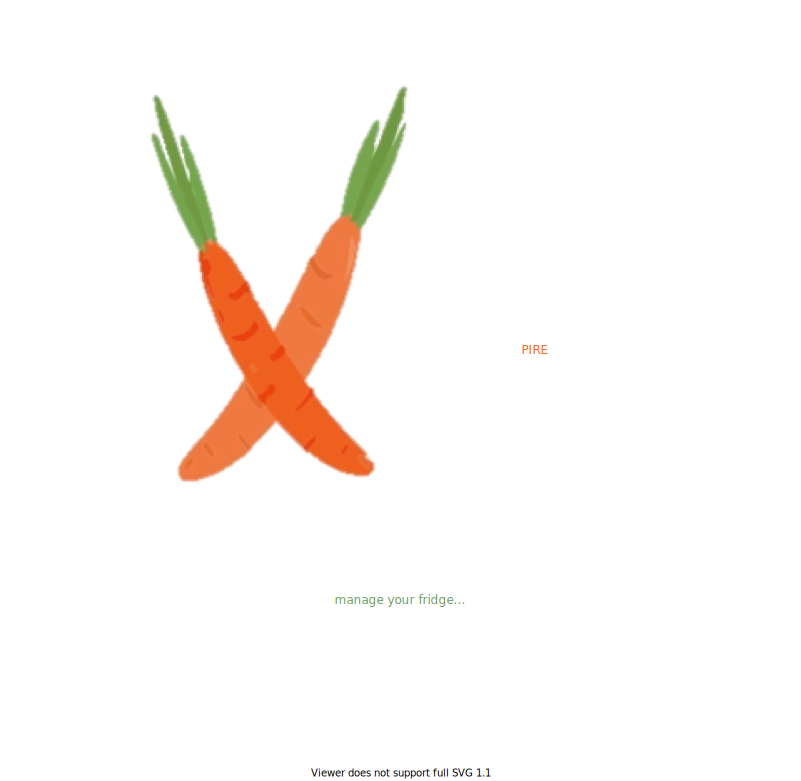
\includegraphics{img/logo.jpg}
\end{minipage}
\vspace{1em}
\sffamily
\begin{center}
	\textsf{\large{}Duale Hochschule Baden-W\"urttemberg\\[1.5mm] Mannheim}\\[2em]
	\textsf{\textbf{Seminararbeit}}\\[8mm]
	\textsf{\textbf{\Large{}Xpire - Dokumentation zum Projekthergang}} \\[1.5cm]
	\textsf{\textbf{\Large{}Studiengang Wirtschaftsinformatik}\\[3mm] \textsf{Studienrichtung Software Engineering}}
	
	\vspace{3em}
%	\textsf{\Large{Sperrvermerk}}
\vfill

\begin{minipage}{\textwidth}

\begin{tabbing}
	Wissenschaftlicher Betreuer: \hspace{0.85cm}\=\kill
	Verfasser: 
		\> Engel, Andrea: xyz \\
		\> Dutzi, Jonas: 6681598 \\
		\> Richarz, Verena: xyz \\
		\> Waage, Felix: 3459154 \\
		\> Werner, Yvonne: 8519757 \\
		\> Westphal, Fabio: 6198411 \\
		\> Zahn, Milena: 7488221 \\\\
	Firma: \> SAP SE \\[1.5mm]
	Kurs: \> WWI 17 SEB\\[1.5mm]
	Studiengangsleiter: \> Prof. Dr. Sebastian Ritterbusch  \\[1.5mm]
	Modul: \> Entwicklung mobiler Applikationen \\[1.5mm]
	Dozent/-in: \> Michael Spengler \\[1.5mm]
	Bearbeitungszeitraum: \> 11.05.2020 - 31.07.2020
	
\end{tabbing}
\end{minipage}

\end{center}

\end{titlepage}

\pagenumbering{roman} % Römische Seitennummerierung
\normalfont

%--------------------------------
% Verzeichnisse - nicht benötige Verzeichnisse bitte auskommentieren / löschen.
%--------------------------------

%   Sperrvermerk
%\input{nondisclosurenotice}

% Ehrenwörtliche Erklärung ewerkl.tex einziehen
% \input{ewerkl.tex}

%	Kurzfassung
% \input{abstract}

%	Inhaltsverzeichnis
\tableofcontents

%	Abbildungsverzeichnis
%\listoffigures

%	Tabellenverzeichnis
% \listoftables

%	Listingsverzeichnis
% \lstlistoflistings

% 	Algorithmenverzeichnis
%\listofalgorithms

% 	Abkürzungsverzeichnis (siehe Datei acronyms.tex!)
% !TEX root =  master.tex

\clearpage
\chapter*{Abkürzungsverzeichnis}	
\addcontentsline{toc}{chapter}{Abkürzungsverzeichnis}


\begin{acronym}
	\acro{DHBW}{Duale Hochschule Baden-Württemberg}
	\acro{PWA}{Progressive Web App}
	\acro{VPC}{Values Proposition Canvas}
	\acro{MVP}{Minimal Viable Product}
	\acro{API}{Application Programming Interface}
	\acro{IndexedDB}{Indexed Database API}
	\acro{API}{Application Programming Interface}
	\acro{HTML}{Hypertext Markup Language}

\end{acronym}


%--------------------------------
% Start des Textteils der Arbeit
%--------------------------------
\clearpage
\ihead{\chaptername~\thechapter} % Neue Header-Definition
\pagenumbering{arabic}  % Arabische Seitenzahlen

%	Anleitungs-Datei anleitung.tex einziehen. Auf diese Weise sollten Sie versuchen, für jedes einzelne
% Kapitel eine eigene Datei anzulegen und mittels input-Kommando einzuziehen.

% !TEX root =  master.tex
\chapter{Einleitung}
% Random commentar
\input{tex/chapter01/1.1.grundidee}
\input{tex/chapter01/1.2.PWA}
% !TEX root =  master.tex
\section{Vorgehensweise}
Um so effektiv wie möglich zusammen zu arbeiten, haben wir uns eine flexible Art der Aufgabenaufteilung überlegt. Dabei sind wir wie folgt vorgegangen: Zunächst haben wir gemeinsam in einer Brainstorming-Session überlegt, welche Funktionalitäten die Xpire-App beinhalten soll, wie sie aussehen soll und welche Technologien wir für die Umsetzung verwenden möchten. Anschließend hat sich jedes Gruppenmitglied selbstständig mit den Grundlagen einer PWA als auch mit der Softwarebibliothek React vertraut gemacht. In einer zweiten Session haben wir gemeinsam die Code-Basis für das Projekt aufgesetzt und spezifische Verantwortungsbereiche im Projekt definiert, zu denen sich jeder, je nach Stärken und Interessen, selbst zuordnen konnte. Dabei ist zu beachten, dass eine Person nicht zwangsläufig nur im eigenen Verantwortungsbereich agieren muss. Jeder darf entsprechend seiner Stärken den Fokus setzen und darüber hinaus weiteren Aufgaben außerhalb seines Schwerpunktes nachgehen und die anderen Team-Mitglieder bei ihren Aufgaben unterstützen. Wichtig ist uns, dass sich jeder im Team wohl fühlt, dem nachgehen kann, worauf er Lust hat und, ganz wichtig, durch Learning-by-Doing ganz viel Neues erlernen kann.\\
Die Schwerpunkte wurden wie folgt eingeteilt:
\begin{itemize}[noitemsep]
	\item \textbf{Design:} Verena, Andrea
	\item \textbf{App-Entwicklung:} Felix, Milena, Yvonne, Verena
	\item \textbf{Datenbank:} Fabio, Jonas
	\item \textbf{Projektmanagement:} Andrea
\end{itemize}
Freitags, an unseren offiziellen Meeting-Terminen, stellen wir einander vor, welche Aufgaben in der Zwischenzeit umgesetzt wurden, definieren neue Aufgaben und reflektieren die bisherige Vorgehensweise. Unter der Woche vereinbaren wir je nach Bedarf individuell Termine mit dem gesamten Team oder treffen uns in Teilgruppen, um bestimmte Aufgaben umzusetzen. Ein Protokoll der Meetings liegt in unserem GitHub-Repository im Dokument \enquote{meetings.md} und kann unter folgendem Link gefunden werden: https://github.com/felixwaage/Xpire/blob/master/meetings.md

Das gesamte Projekt kennzeichnet sich durch eine iterative Arbeitsweise, sodass genug Platz für neue Ideen und Erweiterungen bleibt. Ziel ist es, zunächst ein Minimal-Viable-Product (MVP) zu entwickeln, um ein funktionierendes Produkt liefern zu können, welches sich in zukünftigen Schritten einfach erweitern lässt.



\input{tex/chapter02/chapter02}
\input{tex/chapter02/2.1.VPC}
\input{tex/chapter02/2.2.Benutzer}
% !TEX root =  master.tex
\section{Anforderungsanalyse}
% Funktioale Anforderungen und nicht funktionale Anforderungen
Eine zentrale Fragestellung bei der Konzeption von progressiven Web Apps ist die nach den Zielen der Anwendung. Welche Aufgaben soll der Benutzer erledigen können und welche qualitativen sowie technischen Rahmenbedingungen sollen dabei berücksichtigt werden? Nach diesen Fragen wurde eine Liste von funktionalen und nicht-funktionalen Anforderungen erstellt, welche sich auf die erste Version der Xpire-App, das Minimal Viable Product (MVP), beziehen:

\subsection{Funktionale Anforderungen}
Die funktionalen Anforderungen beschreiben die Funktionalitäten, welche die Anwendung bereitstellen soll:
\begin{itemize}[noitemsep]
	\item[F1] \textbf{Produkte hinterlegen:} Der Kunde soll die Möglichkeit haben, gekaufte Produkte per Barcode-Scan oder manuell hinterlegen zu können.
	\item[F2] \textbf{Produktinformationen hinterlegen:} Der Benutzer hat die Möglichkeit folgende Informationen zu den Produkten zu hinterlegen: Titel, Anzahl, Einkaufsdatum und Gültigkeitsdatum.
	\item[F3] \textbf{Produkte verwalten:} Die Produkte sollen dem Benutzer in übersichtlicher Weise angezeigt werden. Der Nutzer hat die Möglichkeit ein Produkt zu löschen oder die hinterlegten Informationen zu den Produkten jederzeit zu verändern.
	\item[F4] \textbf{Bild hinterlegen:} Benutzer sollen die Möglichkeit haben, pro Produkt ein Bild hochladen zu können.
	\item[F5] \textbf{Benachrichtigungen erhalten:} Der Benutzer soll eine Push-Benachrichtigung erhalten, wenn ein Produkt kurz vor dem Ablauf seiner Haltbarkeit steht.
\end{itemize}

\subsection{Nicht-funktionale Anforderungen}
Die nicht-funktionale Anforderungen betreffen die Umstände, unter denen die geforderten Funktionalitäten zu erbringen sind:

% Welche User-Entwickler Dokumentation wurde bereitgestellt, wo und warum? (Giithub Readme)

\begin{itemize}[noitemsep]
	\item[NF1] \textbf{Usability-Ziele:} Die Usability (dt.: Gebrauchstauglichkeit) ist definiert als das Ausmaß, in dem ein Produkt in einem bestimmten Anwendungskontext genutzt werden kann, um bestimmte Ziele mit geringem Aufwand und hoher Zufriedenheit zu erreichen.\autocite[vgl.][S.3 ff.]{Balzert.2009} Basierend auf den Ergebnissen der Benutzerprofilanalyse wurde
	der Fokus bei der erstellten progressiven Web App auf die Erreichung folgender Kriterien gelegt:
	\begin{itemize}[noitemsep]
	\item[NF1.1] \textbf{Verständliche Informationsstruktur:}Eine klare Informationsstruktur schafft die Voraussetzung für die intuitive Bedienbarkeit des Systems und kann damit grundlegend zu einer positiven Benutzererfahrung beitragen.\autocite[vgl.][S.106 ff.]{Moser.2012} Aus diesem Grund sollen bereitgestellte Informationen möglichst logisch strukturiert und leicht verständlich sein. Grundsätzlich sollten dem Anwender nur die im aktuellen Kontext benötigten Informationen präsentiert und Unwichtiges weggelassen werden.
	\item[NF1.2] \textbf{Durchdachtes Navigationskonzept:}Eine gut gestaltete Navigation erleichtert dem Benutzer die Orientierung und helfen ihm die folgenden Fragen zu beantworten: Wo befinde ich mich, wie bin ich hier hergekommen und wohin kann ich von hier aus gehen?\autocite[vgl.][S.116 ff.]{Moser.2012}
	\end{itemize}
	\item[NF2] \textbf{Technische Rahmenbedingungen:}Aus den technischen Randbedingungen wird in der Regel die Wahl der einzusetzenden Technologien getroffen. Diese sind:
	\begin{itemize}[noitemsep]
		\item[NF2.1] \textbf{Physikalische Nutzungsumgebung:} Einsatzort der PWA kann überall sein. Um eine optimale Lesbarkeit zu garantieren, sollte daher auf die richtige Verwendung von Farbkontrasten und Schriftarten geachtet werden.
		\item[NF2.2] \textbf{Hardware:} Als Endgerät kann sowohl ein Smartphone, als auch ein Tablet oder ein PC verwendet werden. Die PWA muss daher so konzpipiert sein, dass sie auf die Eigenschaften des jeweils benutzten Endgeräts optimal reagieren kann.
	\end{itemize}
\end{itemize}
 
% !TEX root =  master.tex
\section{Monetarisierungsstrategie}
Grundsätzlich gibt es zahlreiche Möglichkeiten, um mit einer App Geld zu verdienen. Wichtig ist, im Vorfeld zu überlegen, wie die App auf dem Markt positioniert werden soll und welche Monetarisierungsstrategie am besten passt. Zu den drei bekanntesten Möglichkeiten zählen:
\begin{itemize}[noitemsep]
	\item \textbf{Paid-App:} Dies ist nicht die einfachste Möglichkeit, um Geld mit einer App zu verdienen. Statt die App kostenlos im Google Play Store oder im Apple Store anzubieten, wird die App kostenpflichtig angeboten, sodass dem Nutzer einmalige Kosten beim Download der App entstehen.
	\item \textbf{In-App-Werbung:} Das Schalten von Werbung innerhalb der App ist eine beliebte Methode um den Umsatz anzukurbeln. Die Möglichkeiten sind sehr vielfältig und reichen von klassischen Werbebannern bis hin zu boomender Videowerbung.
	\item \textbf{Freemium:} Bei dieser Monetarisierungsstrategie ist der Download der App kostenlos, der User hat dann die Möglichkeit durch In-App-Käufe oder einem Abo neue Inhalte, neue Funktionen oder die Laufzeit einer Vollversion zu verlängern. Dafür fallen dem User dann zusätzliche Kosten an.
\end{itemize}
Neben den genannten Beispielen gibt es noch viele weitere Möglichkeiten zur Monetarisierung einer App. Wir haben die verschiedenen Szenarien genauer beleuchtet und sind zu folgender Auswertung gekommen:\\
Eine Paid-App kommt für uns nicht in Frage, da wir die Xpire-App ausschließlich kostenlos anbieten möchten. Unser Ziel ist es, möglichst viele User zu gewinnen um so für mehr Nachhaltigkeit und einen verantwortungsvolleren Umgang mit Lebensmitteln zu sorgen. Nur wenige Benutzer sind bereit, für eine App Geld auszugeben und die Gefahr, das andere Anbieter eine ähnliche, kostenlose Alternative anbieten, ist hoch. Daher scheidet diese Strategie aus.
Das Schalten von Werbung sehen wir als guten Kompromiss, um die App für den User kostenlos zu gestalten und trotzdem Umsatz zu generieren. Falls wir zukünftig Werbung schalten werden, darf diese jedoch weder unseriös, aufdringlich oder nervig wirken und muss gegen Bezahlung deaktiviert werden können.
Das Anbieten von zusätzlichen In-App-Käufen oder das Abschließen eines Abos um auf neue Inhalte oder Funktionen zugreifen zu können, halten wir in unserem Fall jedoch für wenig sinnvoll.\\
Es sind zusätzliche Funktionen wie das Aufzeigen von passenden Angeboten der umliegenden Supermärkte oder das Vorschlagen von Rezepten basierend auf den hinterlegten Produkten geplant. Diese zusätzlichen Funktionen sollen aber keine kostenpflichtigen Features darstellen und ebenfalls kostenlos angeboten werden. Vielmehr halten wir die Kooperation mit verschiedenen Rezeptseiten wie Chefkoch.de oder restegourmet.de als auch die Kooperation mit diversen Supermärkten für sinnvoll. Darüber hinaus besteht die Möglichkeit die App teilweise durch Spenden zu finanzieren und kostenlose Infrastruktur bei verschiedenen Hosting-Anbietern anzufragen, denn einige Anbieter stellen gemeinnützigen Vereinen kostenlosen Speicherplatz zu Verfügung.






\input{tex/chapter03/chapter03}
% !TEX root =  master.tex
\section{Eingesetzte Technologien}
\subsection{React}
React ist eine JavaScript-Bibliothek zur Erstellung von Benutzeroberflächen, die 2013 von Facebook unter BSD-Lizenz veröffentlicht wurde. Zentrales Konzept von React ist die Komponenten-bezogene Architektur, die als Basis für leicht nachvollziehbaren und wartbaren Frontend-Code dient. Komponenten erlauben es, die Benutzeroberfläche in autarke, wiederverwendbare Einheiten aufzuteilen. Dabei kapseln sie Struktur (HTML), Aussehen (CSS) und Logik (JavaScript).\autocite[vgl.][]{?}\\
Neben React stellen Angular oder vue.js vergleichbare Alternativen dar. Wir haben uns als Team jedoch bewusst für die Nutzung von React entschieden aus folgenden Gründen:
\begin{itemize}[noitemsep]
	\item ein Großteil des Teams hat bereits mehr Erfahrungen mit React als mit Angular oder vue.js gesammelt $\rightarrow$ dieser Erfahrungsschatz ermöglicht einen schnellen Einstieg ins Projekt
	\item Es gibt bereits viele Projekte, die React in Verbindung mit einer PWA verwenden $\rightarrow$ liefert Orientierung und hilft beim Verständnis	\item die Anforderungen an Xpire beinhalten keine außergewöhnlichen Ansprüche, welche nicht mit React erfüllt werden könnten
\end{itemize}

\subsection{Datenbank}\label{chapter:datenbank}
Die Prämisse, die gesamte Anwendung light-weight und dezentral zu gestalten, wirkt sich vor allem auch auf die Datenhaltung aus. In der Regel werden bei Web-basierten Anwendungen die Daten, die für spätere Verwendungen zur Verfügung stehen sollen, in einer Datenbank auf einem zentralen Rechner gespeichert. Für die Xpire-App wollten wir aber auf eine solche Zentralisierung verzichten, um zum einen die laufenden Kosten minimal zu halten und zum anderen den höchsten Datenschutz zu gewährleisten, indem die Daten nur auf dem Gerät des Benutzers gespeichert werden. Bei nativen Apps wird hierfür ein Verzeichnis auf dem Gerätespeicher angelegt, in dem sämtliche Dateien und Datenbanken dauerhaft abgelegt werden können. Bei einer \ac{PWA} ist es allerdings nicht vorgesehen, auf dem Dateisystem des jeweiligen Geräts zu operieren, da es sich letztendlich um eine Webseite handelt.\\
Hier bieten moderne Browser einige Möglichkeiten an, Daten lokal zu speichern. Die üblichen Möglichkeiten hierfür sind Cookies, SessionStorage und LocalStorage. Teilweise sind diese aber zeitlich aber vor allem strukturell begrenzt und können so nicht als Ersatz für eine Datenbank herhalten. Abhilfe schaffen kann da die sogenannte IndexedDB, eine Schnittstelle des Browsers für eine primitive Datenbank. So ist es einer Webseite möglich, Daten lokal und nicht serverseitig in einer Datenbank zu speichern. Eine solche Datenbank erlaubt auch Hochleistungssuchen der Daten durch die Verwendung von Indizes.\footnote{\url{https://developer.mozilla.org/de/docs/Web/API/IndexedDB_API}}\\
Um den Zugriff auf die IndexedDB zu vereinfachen nutzen wir die Wrapper-Bibliothek Dexie.\footnote{\url{https://dexie.org}} 
Dexie löst drei Hauptprobleme mit der nativen IndexedDB-API:
Mehrdeutige Fehlerbehandlung, schwache Anfragen und
Code-Komplexität und bietet so eine saubere Datenbank-API, die für unseren Einsatz bestens performt. Angelegte Produkte können hiermit persistiert, abgefragt und geändert werden. Neugierige Nutzer der Xpire-App können über die Entwicklerwerkzeuge ihres Browsers den Inhalt der indizierten Datenbank und somit die gespeicherten Produkte einsehen. 
	
\subsection{Platform}
Für Xpire haben wir ein Repository auf GitHub angelegt, sodass wir die Web App kostenlos über GitHub Pages hosten können. GitHub Pages sind öffentliche Webseiten, die kostenlos über GitHub gehostet werden. GitHub-Benutzer können sowohl persönliche Webseiten als auch Webseiten, die sich auf bestimmte GitHub-Projekte beziehen, erstellen und hosten. Wir haben GitHub Pages aus folgenden gründen für unser Projekt gewählt:
\begin{itemize}[noitemsep]
	\item Es ist kostenlos und ermöglicht ein einfaches Deployment.
	\item Es ist zentral mit dem GitHub Repository verbunden.
	\item Es unterstützt die gemeinsame Entwicklung.
\end{itemize}
Da sich die Xpire-App aktuell in der Entwicklungsphase befindet, ist GitHub Pages eine sehr zufriedenstellende Technologie. Im späteren Verlauf, wenn die App live gehen soll und für Endanwender verfügbar gemacht werden soll, ist GitHub Pages jedoch nicht mehr die geeignetste Wahl für das Hosting. Zu einem späteren Zeitpunkt werden wir ausweichen auf entweder die SAP Cloud Plattform, Amazon AWS oder einen gemieteten Server, beispielsweise von IONOS oder Strato.

\subsection{Sonstiges}
\textbf{Authentifizierung}: Eine Authentifizierung ist derzeit nicht vorhanden und wird, je nach Entwicklung der Funktionalitäten und Bedarf, zu einem späteren Zeitpunkt ergänzt. Falls die technischen Möglichkeiten es zulassen, wollen wir die Web App jedoch ohne Authentifizierung anbieten, da wir keine Daten unser Endnutzer erheben möchte. Für uns stellt der Datenschutz eine höhere Priorität dar.

\textbf{Präsentations- und Feedbackmöglichkeiten:} Präsentations- und Feedbackmöglichkeiten sind in der aktuellen Version der App nicht vorhanden, da sie nicht zu den definierten Anforderungen eines MVP's gehören. Im zukünftigen Live-Betrieb soll die App jedoch Feedbackmöglichkeiten von den Nutzer zur Verfügung stellen, um eine kontinuierlichen, benutzerorientierten Service anbieten zu können. Die Möglichkeiten zur Einholung des Feedbacks sollen den Nutzer in der Anwendung der App jedoch nicht einschränken. Daher sollen es keine willkürlich aufploppende Bewertuns-Popups geben, sondern lediglich einen Feedback-Button, welcher den Nutzer zu einem Feedback-Formular navigiert. Die Abgabe von Feedback erfolgt auf freiwilliger Basis.
	



% !TEX root =  master.tex
\newpage
\section{Konzeptuelles Modell}
% Welche Architektur und Warum?
% User-Authentifizierung?
% Welche Persistierung?
% Welche Tests und warum?

In den vorherigen Abschnitten wurden bereits einige Merkmale der Xpire-App beschrieben. Darauf aufbauend sollen im Folgenden die Zusammenhänge der verschiedenen Bestandteile näher erläutert werden und somit einen detaillierten Überblick über das konzeptionelle Modell liefern.\\
Kern der Xpire-App ist das Frontend, welches mit Hilfe von React als PWA konzipiert ist. Wie den Abbildungen \ref{fig:prot1} und \ref{fig:prot2} entnommen werden kann, besteht die Xpire-App aus 3 Ansichten: \textit{Home-Screen}, \textit{Product-Screen} und dem \textit{Create-Screen}. Diese Ansichten werden in React durch Komponenten realisiert, welche in unterschiedlichen Kontexten wiederverwendet werden können. Der Home-Screen besitzt demzufolge die Komponente AppBar und eine Komponente zur Listendarstellung der Produkte. Die Ansichten \textit{Product-Screen} und \textit{Create-Screen} werden durch dieselbe Komponente realisiert, da zum Erstellen und Anzeigen der Produktinformation ähnliche UI-Bestandteile benötigt werden. Die Darstellung passt sich hierbei automatisch anhand der übergebenen Parameter an. Hierdurch können Code-Duplikate vermieden werden und auch der Raum für Fehler wird reduziert.\\
Ein Weiterer wichtiger Bestandteil der Anwendung ist die IndexedDB, welche zur dauerhaften Persistierung der Daten verwendet wird. Wie bereits in Abschnitt \ref{chapter:datenbank} erwähnt wird hierfür das Modul \textit{Dexie} verwendet. Neben der Datenhaltung in der lokalen Datenbank wird eine aktuelle Kopie der gesamten Datenbank in einem Array im \textit{State} der App-Komponente synchron gehalten, wodurch sowohl die Listen-Komponente als auch die Product-Screen-Komponente darauf zugreifen können.

Der Nutzer soll später seine Produkte mit Hilfe des einheitlichen Barcodes hinzufügen können. Dies soll die Verwendung deutlich beschleunigen und vereinfachen, da so Informationen wie Titel, Gewicht, usw. nicht manuell eingetragen werden müssen. Um die dazu benötigten Informationen zu erhalten, wird die OpenFoodFacts-Api verwendet. Diese führt eine Datenbank mit umfassenden Produktinformationen und kann Anfragen über den Barcode entgegennehmen. Des Weiteren wird diese API verwendet, um Abbildungen der einzelnen Produkte zu erhalten. Dadurch wird dem Nutzer die Verwendung der Anwendung zusätzlich vereinfacht. Darüber hinaus ist in einer späteren Version angedacht, die Produktbilder lokal in der Datenbank zu speichern, um auch bei Offline-Betrieb die Bilder anzeigen zu können.

\subsection{Notifications}
Damit der Nutzer der App diese nicht aktiv öffnen muss, um über demnächst ablaufende Produkte informiert zu werden, ist es sehr sinnvoll, dass die App automatisch Push-Mitteilungen versendet. Moderne Browser können heutzutage solche Benachrichtigungen von Webseiten anzeigen, die hierfür die Notifications-API\footnote{\url{https://developer.mozilla.org/en-US/docs/Web/API/Notifications_API}} nutzen. 
Normalerweise werden solche Push-Nachrichten von einem Server der Webseite ausgelöst. Da unsere Anwendung aber komplett dezentral ausgeführt werden soll, muss eine Möglichkeit gefunden werden, die Notifications on-Device zu triggern. Es genügt nämlich nicht, bei bestimmten Interaktionen über die angebundenen Event-Handler eine Mitteilung auszulösen, sie müssen vielmehr terminiert werden können.\\
Hierzu gibt es im aktuellen Web-Standard keine vorgesehene Funktion, jedoch testet Google ganz aktuell dahingehend eine Erweiterung der Notifications-API.\footnote{\url{https://developers.chrome.com/origintrials/#/view_trial/6883752030435803137}}
Im Rahmen eines sogenannten Origin Trials wird ein sicheres Experimentieren mit neuen Funktionen der Web-Plattform ermöglicht. Um die bestmöglichen Designs zu erzielen, werden solche neuen Funktionen nicht vorzeitig zu De-facto-Standards, auf die sich Webentwickler dann verlassen und eine Abänderung nur schwer möglich machen, sondern sie werden in einem iterativen Prozess getestet und durch Feedback verbessert, bevor sie letztendlich in den Standard ausgerollt werden.
So sollte es im Idealfall einfacher sein, neue Funktionen freizulegen und zu iterieren, aber die Versuchspopulation zuverlässig einzuschränken. Mit einer Testpopulation von Entwicklern, die sich verpflichtet haben, Feedback zu geben, und Begrenzungen in der Größe der Anwenderbasis und der Versuchsdauer kann die Iteration schneller erfolgen, aber ohne das Risiko eines sogenannten Burn-in, also einer Resistenz gegen Veränderungen.
Nun haben wir also ein zeitlich begrenztes Token von Google angefordert, um die Funktion \emph{Notification Triggers}\footnote{\url{https://github.com/rknoll/notification-triggers}} für unsere Webapp freizuschalten. Dieses wird im \texttt{<head>}-Tag der \ac{HTML}-Seite mitgegeben. Zusätzlich muss, da wir React verwenden, dem Compiler per ESLint-Befehl mitgeteilt werden, dass Undef-Fehler für die verwendete Klasse \texttt{TimestampTrigger} ignoriert werden sollen, schließlich ist sie noch nicht Teil des Standards, wird aber von Chrome 80+ entsprechend erkannt. Mit dieser Beta-Funktion ist es dann möglich, einen Zeitstempel für das Feuern einer Mitteilung festzulegen und im Service-Worker zu registrieren.\footnote{\url{https://web.dev/notification-triggers/}} Somit ist es uns gelungen, für jedes Produkt einen Alarm zu setzen, der rechtzeitig vor Verfall den User per Push-Mitteilung informiert.
% !TEX root =  master.tex
\section{Entwicklung von Prototypen}
\subsection{Figma}
Zur Erstellung der Prototypen haben wir das Design-Tool \enquote{Figma} verwendet. Dies ist ein Kollaborations-Tool für Designer und funktioniert ähnlich wie Sketch oder Adobe XD, zeichnet sich aber durch zwei signifikante Unterschiede aus\autocite[vgl.][]{?}:
\begin{itemize}[noitemsep]
	\item Es läuft zu 100 \% in Ihrem Browser (keine Installation nötig)
	\item Möglichkeit der Kollaboration mit anderen Personen in Echtzeit
\end{itemize}
Dadurch liefert Figma viele Vorteile, die das gemeinsame Erstellen von Prototypen stark verbessern. Das Tool ist von Designern für Designer entwickelt wurden und einfach im handling. Benutzeroberflächen lassen sich schnell und effektiv designen, ohne viel Zeit in die Einarbeitung des Tools investieren zu müssen. Das kollaboratives Arbeiten in Echtzeit ermöglicht die unkomplizierte Zusammenarbeit am selben Entwurf, ohne extra ein Tool zu installieren oder sich physisch treffen zu müssen. Des weiteren bietet Figma die Möglichkeit, erstellte Screens in vier verschiedenen Formaten zu exportieren als auch Interaktionen hinzuzufügen, um das Projekt im Live-Preview betrachten zu können. Im Live-Preview lassen sich alle zuvor definierten Interaktionen, wie beispielsweise das Navigieren auf einen anderen Screen, ausprobieren und imitieren das Feeling einer echten Anwendung.

\subsection{Mobile First}
Da unsere Zielgruppe eine breite Masse an Menschen beinhaltet, haben wir wert darauf gelegt, dass Xpire möglichst einfach und unkompliziert verwendet werden kann. Einem ansprechenden User Interface sowie einer intuitive User Experience werden daher besondere Bedeutung zugeschrieben.\\
Im Jahr 2015 meldete Google erstmals, dass mehr Suchanfragen über mobile Endgeräte als über Desktop-Geräte erfolgten. Seitdem steigt die der Anteil der Internetnutzer, die auch mit dem Smartphone online gehen, rapide. \footnote{\url{https://de.statista.com/statistik/daten/studie/633698/umfrage/anteil-der-mobilen-internetnutzer-in-deutschland/}} Resultierende aus dieser Entwicklung ist die Wahl des Mobile-First-Ansatzes selbsterklärend. Inzwischen ist nicht mobil-optimierter (responsive) Content ist kaum noch vorstellbar. Mobile Frist lässt sich als neuer Denkansatz im Webdesign definieren. Das Design einer Website wird dabei erstmal in der mobilen Version optimiert, bevor es für größere Bildschirme entwickelt wird. Man arbeitet also von der kleinsten Layout-Version hin zur größten.\autocite[vgl.][]{?}

% Schrittfolge der Screens erklären
\begin{figure}[hbt!]
	\centering
	\includegraphics[width=1.0\textwidth]{img/Prototype_01.pdf}
	\caption{Xpire Welcome-Screen und Home-Screen}
	\label{fig:prot1}
\end{figure}
Die Abbildung \ref{fig:prot1} zeigt den \textit{Welcome-Screen} und den \textit{Home-Screen} der Xpire-App. Der \textit{Welcome-Screen} zeigt das Xpire-Logo, welches mit dem vektorbasierten Grafik- und Zeichenprogramm \enquote{Adobe Illustrator} erstellt wurde. Daher kann es in unterschiedlichen Formaten exportiert und schnell angepasst oder verändert werden. Die gewählte Farbkombination als auch die verwendete Symbolik verleihen dem Logo einen hohen Wiedererkennungswert und ein gewisses Öko-Flair. Das Motto \enquote{Manage your fridge \& get rich} ist nicht nur ein einprägsamer Reim, der sich gut als Werbespruch verwenden lässt, gleichzeitig stellt er eine Anspielung der monetären Ersparnisse dar, die man durch die Benutzung der Xpire-App erzielen kann.\\
Der \textit{Home-Screen} in Abbildung \ref{fig:prot1} zeigt die aktuell hinterlegten Produkte mit Bild, Produktnamen, Verfallsdatum und einer farbigen Statusbar. Ist die Statusbar grün, bedeutet das, dass das Produkt noch haltbar ist und auch nicht unmittelbar vor dem Ablauf der Haltbarkeit steht. Ist der Balken gelb, wie im Mockup bei der \enquote{Milbona Schlagsahne} bedeutet dies, dass das Produkt kurz vor dem Ablauf der Haltbarkeit steht. Wechselt ein Produkt in den gelben Status, erhält der Benutzer eine Push-Notification, mit dem entsprechenden Hinweis zum Haltbarkeitsablauf des jeweiligen Produktes. Ist der Balken rot gefärbt, hat das Produkt das entsprechende Verfallsdatum bereits erreicht oder sogar überschritten.\\
Der \textit{Delete-Screen} zeigt, wie man ein Produkt durch wischen nach links löschen kann. Da sich die Anforderungen an die Bedienbarkeit in der Desktop-Version von der Smartphone-Version unterscheiden, gibt es zum Löschen eines Produktes in der Desktop-Version ein Mülleimer-Icon.
Wird im \textit{Home-Screen} ein Produkt angeklickt, so wird der Nutzer zum \textit{Product-Screen} des jeweiligen Produktes geleitet. Diese Ansicht enthält Details zum Produkt, wie Name, Anzahl, Einkaufdatum und Verfallsdatum und erlaubt dem Nutzer ein Bild des Produktes zu hinterlegen. Alle hinterlegten Informationen lassen sich in dieser Ansicht vom Nutzer ändern.


\begin{figure} 
	\centering
	\includegraphics[width=1.0\textwidth]{img/Prototpye_02.pdf}
	\caption{Xpire Delete-Screen und Product-Screen}
	\label{fig:prot2}
\end{figure}

% !TEX root =  master.tex
\chapter{Präsentation der PWA}
In diesem Kapitel wird die umgesetzte PWA, die zuvor durch Mockups dargestellt wurde, vorgestellt. Da die Grundlagen zur Technologie bereits im Kapitel 3 ausführlich erläutert worden sind, wird hier nicht mehr näher auf die Implementierungsdetails eingegangen,
sondern lediglich das Resultat anhand von Screenshots vorgestellt. Abschließend findet noch ein Abgleich mit den zuvor definierten Anforderungen statt.

Die Umsetzung der PWA erfolgte mithilfe der JavaScript-
Bibliothek React auf Basis des entwickelten Prototypen. Im Folgenden wird der aktuelle Entwicklungsstand
der App näher vorgestellt. Dabei wird auf die Gestaltung
und die Navigation als auch auf die Funktionalität der PWA eingegangen.

\begin{figure}[h!]
	\centering
	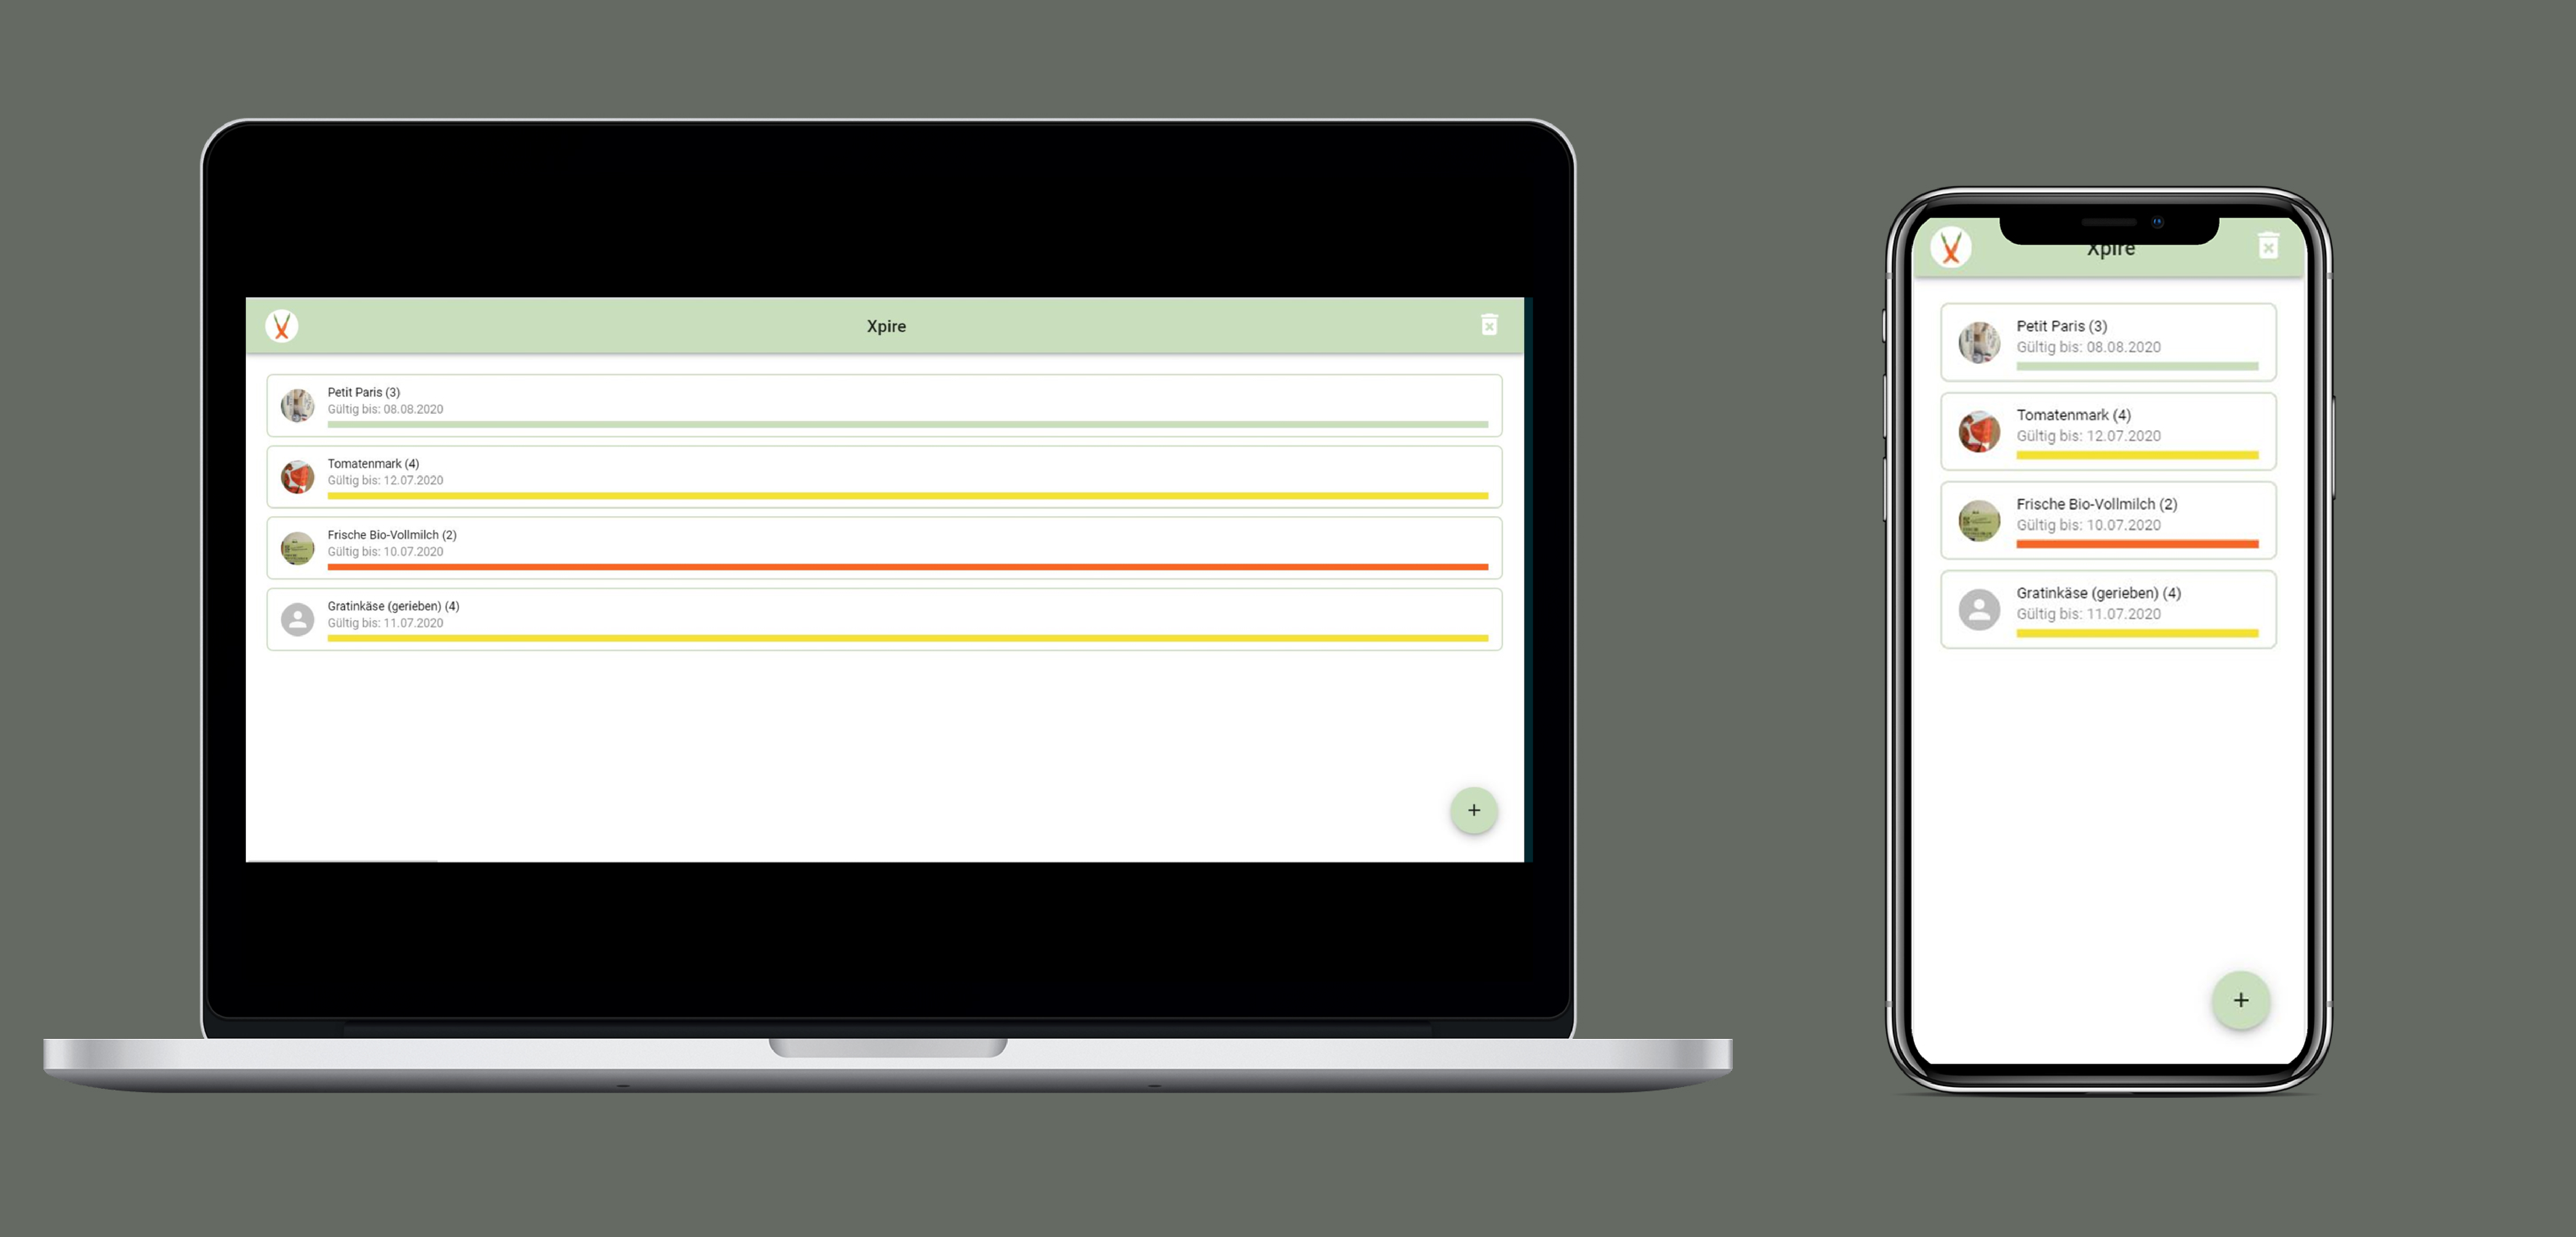
\includegraphics[width=1.0\textwidth]{img/app.pdf}
	\caption{Xpire auf Laptop vs. Smartphone}
	\label{fig:app}
\end{figure}

%\begin{wrapfigure}{r}{0.5\textwidth}
%	\vspace{-1.5\baselineskip}
%	\begin{center}
%		
\includegraphics[width=0.50\textwidth]{img/plus.jpg}
%	\end{center}
%	\setcapindent{0cm}
%	\caption{Ausschnitt des ungerichteten Graphen zum %Einkauf-Problem}
%	\label{fig:graph_edeka}
%\end{wrapfigure}

Die Abbildung \ref{fig:app} zeigt, wie sich die Xpire-App verschiedenen Bildschirmgrößen problemlos anpasst. Zu sehen ist der \textit{Home-Screen} mit eine Auswahl an Beispiel-Produkten sowohl auf dem Laptop als auch auf dem Smartphone.\\
Um Xpire auf dem Laptop zu installieren, muss man folgenden Link in die Adresszeile seines Browsers eingeben: https://felixwaage.github.io/Xpire/. Es erscheint die App,  wie zu sehen in Abbildung \ref{fig:install} im Browser und lässt sich über ein "+" ganz rechts in der Adresszeile als App dem Desktop hinzufügen. Nach einem Klick auf den Plus-Button öffnet sich ein Pop-Up, welches welches es dem Nutzer ermöglicht, die Installation durchzuführen. Klick man den Installations-Button, wird im dritten Schritt die Xpire-App auf dem Desktop hinterlegt, siehe \ref{fig:install}.

\begin{figure}[h!]
	\centering
	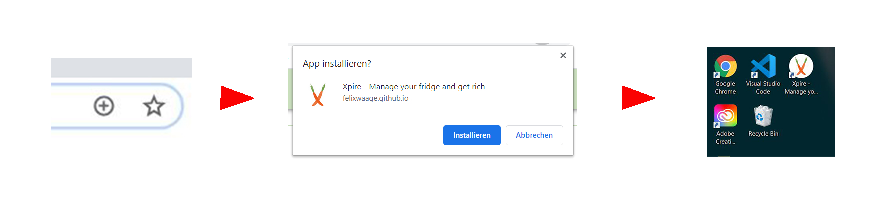
\includegraphics[width=1.1\textwidth]{img/install.pdf}
	\caption{Xpire-Installationsprozess am Laptop}
	\label{fig:install}
\end{figure}

Die Installation auf dem Smartphone erfolgt äquivalent zu der auf dem Desktop. Nach dem Öffnen des Links wid über ein Pop-Up die Möglichkeit zur Installation bereit gestellt. Xpire wird dann auf dem Smartphone angezeigt wie eine native mobile App und weist auch nach dem Öffnen keine Unterschiede zu einer nativen App auf. Dennoch läuft die App als PWA komplett im Browser. 

% was ist unterschiedlich im Vergleich zu den Mockups?
Die Gestaltung als auch der User-Flow der entwickelten PWA entsprechen fast eins zu eins dem der Mockups. Geringe Unterschiede lassen sich an folgenden Punkten feststellen:
 \begin{itemize}[noitemsep]
 	\item \textbf{AppBar:} Das Logo in der entwickelten PWA hat einen weißen Kreis als Hintergrund. Das Icon oben recht ist nicht wie im Mockup ein Zahnrad, sondern ein weißes Mülleimer-Icon.
 	\item \textbf{Produkt löschen:} Die Produkte lassen sich einzeln nicht direkt im \textit{Home-Screen} per Wischen nach links, wie designed im Mockup, löschen, sondern lediglich im \textit{Produkt-Screen} über ein Mülleimer-Icon. Wird jedoch das Mülleimer-Icon oben rechts in der AppBar des \textit{Home-Screen} dar, erhält der Nutzer die Möglichkeit, alle hinterlegten Produkte auf einmal zu löschen.
 	\item \textbf{Produkte verwalten:} Der \textit{Produkt-Screen} wurde implementiert, so wie er im Mockup designed wurde. Das hinterlegte Bild wird angezeigt und Name, Anzahl, Einkaufsdatum und Ablaufdatum lassen sich durch das Anklicken des jeweiligen Textfeldes ändern. Lediglich die Terminologie des Buttons hat wurde von \enquote{Speichern} zu \enquote{Ändern} verändert.
 \end{itemize}

%neuer Screen: Produkt hinzufügen 
Neben der Umsetzung des erstellten Mockups, wurde zusätzlich eine Ansicht zum Hinzufügen eines neuen Produktes entwickelt, zu sehen in Abbildung \ref{fig:add}. Der Nutzer hat die Möglichkeit einen Barcode zu scannen oder ihn manuell im Barcode-Textfeld einzugeben. Über die OpenFood-API wird automatisch das jeweilige Produktbild angezeigt und der Titel im dazugehörigen Feld angezeigt.

\begin{figure}[h!]
	\centering
	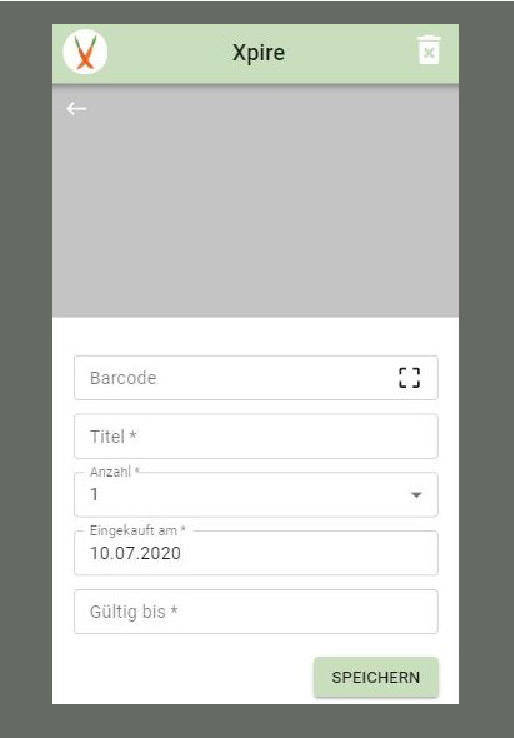
\includegraphics[width=0.6\textwidth]{img/add.pdf}
	\caption{Produkt hinzufügen}
	\label{fig:add}
\end{figure}

Die Standard-Anzahl der Produkte beträgt 1, lässt sich aber über ein Dropdown einfach erhöhen. In dem Eingabefeld für das Einkaufsdatum ist automatisch das aktuelle Datum vorausgewählt, was sich jedoch ändern lässt, sobald man in das Textfeld reinklickt. Es öffnet sich ein Date-Picker, genau wie bei der Eingabe des Gültigkeitsdatums. Nach dem Speichern wird das Produkt automatisch dem \textit{Home-Screen} hinzugefügt.


% Tests --> feingarnulare Unit Tests, acceptance tests?

% Deployment

% !TEX root =  master.tex
\newpage
\section{Anforderungsabgleich}
In diesem Abschnitt wird betrachtet, welche Vorgaben der Spezifikation aus Kapitel 2.3 realisiert werden konnten. Die Bewertung des Erfüllungsgrads sowie die Beschreibung beziehen sich hierbei lediglich auf den aktuellen Stand der Implementierung.

\subsection{Abgleich der funktionalen Anforderungen}

\begin{tabular}{lcp{12.3cm}}
	\textbf{Nr.} & \textbf{Erfüllt} & \textbf{Beschreibung}\\
	\hline
	F1 & Ja & Auf der Ansicht \textit{Product-Screen} hat der Nutzer die Möglichkeit, gekaufte Produkte per Barcodenummer einzugeben. Daraufhin wird automatisch das dazugehörige Produktbild angezeigt.\\
	F2 & Ja &  Der App-User kann im \textit{Product-Screen} nicht nur das Bild hochladen und ändern, er hat auch die Möglichkeit alle hinterlegten Produktinformationen (Name, Anzahl, Einkaufsdatum, Verfallsdatum) zu ändern.\\
	F3 & Ja &  Auf dem \textit{Home-Screen} werden dem Benutzer alle hinterlegen Produkte übersichtlich angezeigt und er hat die Möglichkeit diese zu verwalten, also Produkte zu löschen oder Produktinformationen zu verändern.\\
	F4 & Teils &  Der Benutzer kann manuell kein Bild hochladen. Jedoch wird ihm ein Bild seine Produktes angezeigt, sobald er den Barcode einscannt oder den Code manuell in das dafür vorgesehene Eingabefeld auf dem \textit{Product-Screen} eingibt.\\
	F5 & Ja &  Ist ein Produkt nur noch 3 Tage haltbar, erhält der User eine Push-Notification, um an das zeitnahe Verbrauchen dieses Produktes erinnert zu werden.\\
	\hline
\end{tabular}

\subsection{Abgleich der nicht-funktionalen Anforderungen}

\begin{tabular}{lcp{12.3cm}}
	\textbf{Nr.} & \textbf{Erfüllt} & \textbf{Beschreibung}\\
	\hline
	NF1.1 & Ja & Informationen wurden möglichst sinnvoll strukturiert, bezeichnet und dargeboten.\\
	NF1.2 & Ja & Die Navigation wurde so konzipiert, dass sie dem Benutzer Orientierung auf jeder Ansicht innerhalb der App bietet. Durch unterschiedliche Farbgebungen werden auf visuelle Art und Weise zusätzlich Informationen zum Status der Haltbarkeit eines Lebensmittels vermittelt.\\
	NF2.1 & Ja & Zur Erhöhung der Lesbarkeit wurde auf eine kontrastreiche Darstellung geachtet und eine gut leserliche und Browser-kompatible Schriftart gewählt.\\
	NF2.2 & Ja & Die PWA passt sich an die geforderten Bildschirmgrößen an. Durch den Mobile-First-Ansatz wirkt sie optische wie eine native mobile Applikation, passt sich aber auch problemlos der Bildschirmgröße eines Tablets oder Desktops an.\\
	\hline
\end{tabular}
% !TEX root =  master.tex
\chapter{Zusammenfassung und Ausblick}

% Was könnten nächste Schritte sein? Wie könnte die App erweitert werden?

% Was passiert, wenn man ein Produkt löscht? Ist es dann in der Datenbank geschlöscht oder wird nur ein Attribut gesetzt? Welche Auswirkungen hätten diese Möglichkeiten?

% Was waren unsere Learnings?


%	Literaturverzeichnis
\ihead{} % Neue Header-Definition
\printbibliography
\cleardoublepage

% Der Anhang beginnt hier - jedes Kapitel wird alphabetisch aufgezählt. (Anhang A, B usw.)
\appendix
\ihead{\appendixname~\thechapter} % Neue Header-Definition

% appendix.tex einziehen
\input{appendix}


\end{document}
